% Created by tikzDevice version 0.12
% !TEX encoding = UTF-8 Unicode
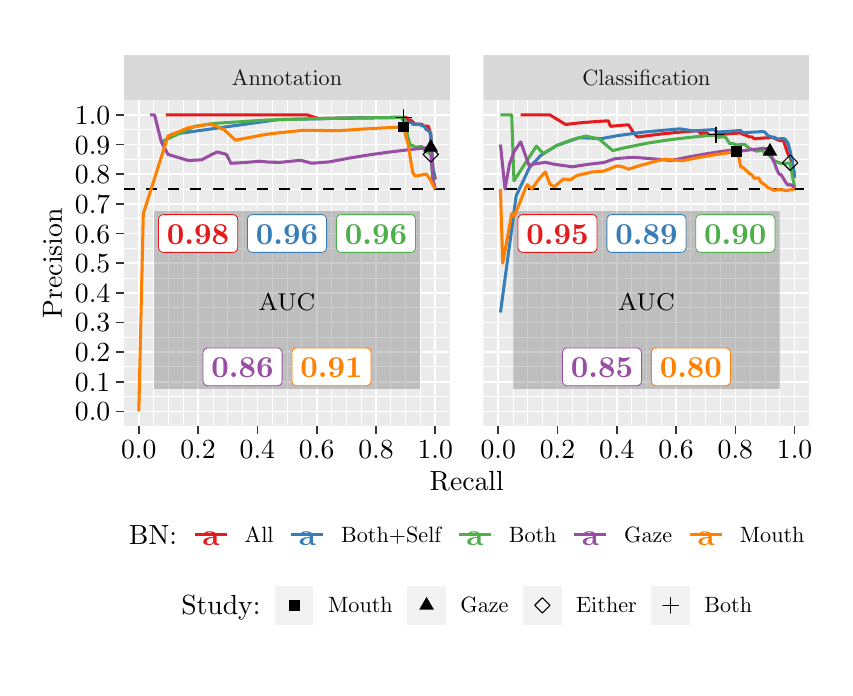
\begin{tikzpicture}[x=1pt,y=1pt]
\definecolor{fillColor}{RGB}{255,255,255}
\path[use as bounding box,fill=fillColor,fill opacity=0.00] (0,0) rectangle (288.00,231.38);
\begin{scope}
\path[clip] (  0.00,  4.41) rectangle (288.00,226.97);
\definecolor{drawColor}{RGB}{255,255,255}
\definecolor{fillColor}{RGB}{255,255,255}

\path[draw=drawColor,line width= 0.6pt,line join=round,line cap=round,fill=fillColor] (  0.00,  4.41) rectangle (288.00,226.97);
\end{scope}
\begin{scope}
\path[clip] ( 34.81, 87.39) rectangle (152.63,205.21);
\definecolor{fillColor}{gray}{0.92}

\path[fill=fillColor] ( 34.81, 87.39) rectangle (152.63,205.21);
\definecolor{drawColor}{RGB}{255,255,255}

\path[draw=drawColor,line width= 0.3pt,line join=round] ( 34.81, 98.10) --
	(152.63, 98.10);

\path[draw=drawColor,line width= 0.3pt,line join=round] ( 34.81,108.81) --
	(152.63,108.81);

\path[draw=drawColor,line width= 0.3pt,line join=round] ( 34.81,119.52) --
	(152.63,119.52);

\path[draw=drawColor,line width= 0.3pt,line join=round] ( 34.81,130.23) --
	(152.63,130.23);

\path[draw=drawColor,line width= 0.3pt,line join=round] ( 34.81,140.94) --
	(152.63,140.94);

\path[draw=drawColor,line width= 0.3pt,line join=round] ( 34.81,151.66) --
	(152.63,151.66);

\path[draw=drawColor,line width= 0.3pt,line join=round] ( 34.81,162.37) --
	(152.63,162.37);

\path[draw=drawColor,line width= 0.3pt,line join=round] ( 34.81,173.08) --
	(152.63,173.08);

\path[draw=drawColor,line width= 0.3pt,line join=round] ( 34.81,183.79) --
	(152.63,183.79);

\path[draw=drawColor,line width= 0.3pt,line join=round] ( 34.81,194.50) --
	(152.63,194.50);

\path[draw=drawColor,line width= 0.3pt,line join=round] ( 45.52, 87.39) --
	( 45.52,205.21);

\path[draw=drawColor,line width= 0.3pt,line join=round] ( 50.87, 87.39) --
	( 50.87,205.21);

\path[draw=drawColor,line width= 0.3pt,line join=round] ( 56.23, 87.39) --
	( 56.23,205.21);

\path[draw=drawColor,line width= 0.3pt,line join=round] ( 66.94, 87.39) --
	( 66.94,205.21);

\path[draw=drawColor,line width= 0.3pt,line join=round] ( 72.30, 87.39) --
	( 72.30,205.21);

\path[draw=drawColor,line width= 0.3pt,line join=round] ( 77.65, 87.39) --
	( 77.65,205.21);

\path[draw=drawColor,line width= 0.3pt,line join=round] ( 88.36, 87.39) --
	( 88.36,205.21);

\path[draw=drawColor,line width= 0.3pt,line join=round] ( 93.72, 87.39) --
	( 93.72,205.21);

\path[draw=drawColor,line width= 0.3pt,line join=round] ( 99.07, 87.39) --
	( 99.07,205.21);

\path[draw=drawColor,line width= 0.3pt,line join=round] (109.79, 87.39) --
	(109.79,205.21);

\path[draw=drawColor,line width= 0.3pt,line join=round] (115.14, 87.39) --
	(115.14,205.21);

\path[draw=drawColor,line width= 0.3pt,line join=round] (120.50, 87.39) --
	(120.50,205.21);

\path[draw=drawColor,line width= 0.3pt,line join=round] (131.21, 87.39) --
	(131.21,205.21);

\path[draw=drawColor,line width= 0.3pt,line join=round] (136.56, 87.39) --
	(136.56,205.21);

\path[draw=drawColor,line width= 0.3pt,line join=round] (141.92, 87.39) --
	(141.92,205.21);

\path[draw=drawColor,line width= 0.6pt,line join=round] ( 34.81, 92.74) --
	(152.63, 92.74);

\path[draw=drawColor,line width= 0.6pt,line join=round] ( 34.81,103.45) --
	(152.63,103.45);

\path[draw=drawColor,line width= 0.6pt,line join=round] ( 34.81,114.17) --
	(152.63,114.17);

\path[draw=drawColor,line width= 0.6pt,line join=round] ( 34.81,124.88) --
	(152.63,124.88);

\path[draw=drawColor,line width= 0.6pt,line join=round] ( 34.81,135.59) --
	(152.63,135.59);

\path[draw=drawColor,line width= 0.6pt,line join=round] ( 34.81,146.30) --
	(152.63,146.30);

\path[draw=drawColor,line width= 0.6pt,line join=round] ( 34.81,157.01) --
	(152.63,157.01);

\path[draw=drawColor,line width= 0.6pt,line join=round] ( 34.81,167.72) --
	(152.63,167.72);

\path[draw=drawColor,line width= 0.6pt,line join=round] ( 34.81,178.43) --
	(152.63,178.43);

\path[draw=drawColor,line width= 0.6pt,line join=round] ( 34.81,189.15) --
	(152.63,189.15);

\path[draw=drawColor,line width= 0.6pt,line join=round] ( 34.81,199.86) --
	(152.63,199.86);

\path[draw=drawColor,line width= 0.6pt,line join=round] ( 40.16, 87.39) --
	( 40.16,205.21);

\path[draw=drawColor,line width= 0.6pt,line join=round] ( 61.58, 87.39) --
	( 61.58,205.21);

\path[draw=drawColor,line width= 0.6pt,line join=round] ( 83.01, 87.39) --
	( 83.01,205.21);

\path[draw=drawColor,line width= 0.6pt,line join=round] (104.43, 87.39) --
	(104.43,205.21);

\path[draw=drawColor,line width= 0.6pt,line join=round] (125.85, 87.39) --
	(125.85,205.21);

\path[draw=drawColor,line width= 0.6pt,line join=round] (147.27, 87.39) --
	(147.27,205.21);
\definecolor{drawColor}{RGB}{0,0,0}

\path[draw=drawColor,line width= 0.6pt,dash pattern=on 4pt off 4pt ,line join=round] ( 34.81,173.08) -- (152.63,173.08);
\definecolor{fillColor}{RGB}{89,89,89}

\path[fill=fillColor,fill opacity=0.30] ( 45.52,100.78) rectangle (141.92,165.04);

\node[text=drawColor,anchor=base,inner sep=0pt, outer sep=0pt, scale=  1.10] at ( 93.72,129.11) {\footnotesize{AUC}};
\definecolor{drawColor}{RGB}{255,127,0}
\definecolor{fillColor}{RGB}{255,255,255}

\path[draw=drawColor,line width= 0.3pt,line join=round,line cap=round,fill=fillColor] ( 97.30,101.99) --
	(122.27,101.99) --
	(122.20,101.99) --
	(122.49,102.00) --
	(122.77,102.06) --
	(123.05,102.16) --
	(123.30,102.31) --
	(123.52,102.49) --
	(123.72,102.71) --
	(123.87,102.96) --
	(123.99,103.22) --
	(124.06,103.51) --
	(124.08,103.80) --
	(124.08,103.80) --
	(124.08,113.82) --
	(124.08,113.82) --
	(124.06,114.11) --
	(123.99,114.40) --
	(123.87,114.66) --
	(123.72,114.91) --
	(123.52,115.13) --
	(123.30,115.31) --
	(123.05,115.46) --
	(122.77,115.56) --
	(122.49,115.62) --
	(122.27,115.63) --
	( 97.30,115.63) --
	( 97.52,115.62) --
	( 97.23,115.63) --
	( 96.94,115.59) --
	( 96.66,115.51) --
	( 96.39,115.39) --
	( 96.16,115.22) --
	( 95.95,115.02) --
	( 95.77,114.79) --
	( 95.64,114.53) --
	( 95.54,114.26) --
	( 95.50,113.97) --
	( 95.49,113.82) --
	( 95.49,103.80) --
	( 95.50,103.94) --
	( 95.50,103.65) --
	( 95.54,103.36) --
	( 95.64,103.09) --
	( 95.77,102.83) --
	( 95.95,102.60) --
	( 96.16,102.40) --
	( 96.39,102.23) --
	( 96.66,102.11) --
	( 96.94,102.03) --
	( 97.23,101.99) --
	cycle;
\end{scope}
\begin{scope}
\path[clip] ( 34.81, 87.39) rectangle (152.63,205.21);
\definecolor{drawColor}{RGB}{255,127,0}

\node[text=drawColor,anchor=base,inner sep=0pt, outer sep=0pt, scale=  1.10] at (109.79,105.00) {\bfseries 0.91};
\definecolor{drawColor}{RGB}{152,78,163}
\definecolor{fillColor}{RGB}{255,255,255}

\path[draw=drawColor,line width= 0.3pt,line join=round,line cap=round,fill=fillColor] ( 65.16,101.99) --
	( 90.14,101.99) --
	( 90.07,101.99) --
	( 90.36,102.00) --
	( 90.64,102.06) --
	( 90.91,102.16) --
	( 91.16,102.31) --
	( 91.39,102.49) --
	( 91.58,102.71) --
	( 91.74,102.96) --
	( 91.85,103.22) --
	( 91.92,103.51) --
	( 91.94,103.80) --
	( 91.94,103.80) --
	( 91.94,113.82) --
	( 91.94,113.82) --
	( 91.92,114.11) --
	( 91.85,114.40) --
	( 91.74,114.66) --
	( 91.58,114.91) --
	( 91.39,115.13) --
	( 91.16,115.31) --
	( 90.91,115.46) --
	( 90.64,115.56) --
	( 90.36,115.62) --
	( 90.14,115.63) --
	( 65.16,115.63) --
	( 65.38,115.62) --
	( 65.09,115.63) --
	( 64.80,115.59) --
	( 64.52,115.51) --
	( 64.26,115.39) --
	( 64.02,115.22) --
	( 63.81,115.02) --
	( 63.64,114.79) --
	( 63.50,114.53) --
	( 63.41,114.26) --
	( 63.36,113.97) --
	( 63.36,113.82) --
	( 63.36,103.80) --
	( 63.36,103.94) --
	( 63.36,103.65) --
	( 63.41,103.36) --
	( 63.50,103.09) --
	( 63.64,102.83) --
	( 63.81,102.60) --
	( 64.02,102.40) --
	( 64.26,102.23) --
	( 64.52,102.11) --
	( 64.80,102.03) --
	( 65.09,101.99) --
	cycle;
\end{scope}
\begin{scope}
\path[clip] ( 34.81, 87.39) rectangle (152.63,205.21);
\definecolor{drawColor}{RGB}{152,78,163}

\node[text=drawColor,anchor=base,inner sep=0pt, outer sep=0pt, scale=  1.10] at ( 77.65,105.00) {\bfseries 0.86};
\definecolor{drawColor}{RGB}{77,175,74}
\definecolor{fillColor}{RGB}{255,255,255}

\path[draw=drawColor,line width= 0.3pt,line join=round,line cap=round,fill=fillColor] (113.36,150.19) --
	(138.34,150.19) --
	(138.27,150.19) --
	(138.56,150.20) --
	(138.84,150.26) --
	(139.11,150.37) --
	(139.37,150.51) --
	(139.59,150.69) --
	(139.78,150.91) --
	(139.94,151.16) --
	(140.05,151.43) --
	(140.12,151.71) --
	(140.15,152.00) --
	(140.15,152.00) --
	(140.15,162.03) --
	(140.15,162.03) --
	(140.12,162.32) --
	(140.05,162.60) --
	(139.94,162.87) --
	(139.78,163.11) --
	(139.59,163.33) --
	(139.37,163.51) --
	(139.11,163.66) --
	(138.84,163.76) --
	(138.56,163.82) --
	(138.34,163.83) --
	(113.36,163.83) --
	(113.58,163.82) --
	(113.29,163.83) --
	(113.00,163.80) --
	(112.72,163.71) --
	(112.46,163.59) --
	(112.22,163.42) --
	(112.01,163.22) --
	(111.84,162.99) --
	(111.70,162.73) --
	(111.61,162.46) --
	(111.56,162.17) --
	(111.56,162.03) --
	(111.56,152.00) --
	(111.56,152.14) --
	(111.56,151.85) --
	(111.61,151.57) --
	(111.70,151.29) --
	(111.84,151.03) --
	(112.01,150.80) --
	(112.22,150.60) --
	(112.46,150.43) --
	(112.72,150.31) --
	(113.00,150.23) --
	(113.29,150.19) --
	cycle;
\end{scope}
\begin{scope}
\path[clip] ( 34.81, 87.39) rectangle (152.63,205.21);
\definecolor{drawColor}{RGB}{77,175,74}

\node[text=drawColor,anchor=base,inner sep=0pt, outer sep=0pt, scale=  1.10] at (125.85,153.20) {\bfseries 0.96};
\definecolor{drawColor}{RGB}{55,126,184}
\definecolor{fillColor}{RGB}{255,255,255}

\path[draw=drawColor,line width= 0.3pt,line join=round,line cap=round,fill=fillColor] ( 81.23,150.19) --
	(106.21,150.19) --
	(106.13,150.19) --
	(106.42,150.20) --
	(106.71,150.26) --
	(106.98,150.37) --
	(107.23,150.51) --
	(107.46,150.69) --
	(107.65,150.91) --
	(107.81,151.16) --
	(107.92,151.43) --
	(107.99,151.71) --
	(108.01,152.00) --
	(108.01,152.00) --
	(108.01,162.03) --
	(108.01,162.03) --
	(107.99,162.32) --
	(107.92,162.60) --
	(107.81,162.87) --
	(107.65,163.11) --
	(107.46,163.33) --
	(107.23,163.51) --
	(106.98,163.66) --
	(106.71,163.76) --
	(106.42,163.82) --
	(106.21,163.83) --
	( 81.23,163.83) --
	( 81.45,163.82) --
	( 81.16,163.83) --
	( 80.87,163.80) --
	( 80.59,163.71) --
	( 80.33,163.59) --
	( 80.09,163.42) --
	( 79.88,163.22) --
	( 79.70,162.99) --
	( 79.57,162.73) --
	( 79.48,162.46) --
	( 79.43,162.17) --
	( 79.42,162.03) --
	( 79.42,152.00) --
	( 79.43,152.14) --
	( 79.43,151.85) --
	( 79.48,151.57) --
	( 79.57,151.29) --
	( 79.70,151.03) --
	( 79.88,150.80) --
	( 80.09,150.60) --
	( 80.33,150.43) --
	( 80.59,150.31) --
	( 80.87,150.23) --
	( 81.16,150.19) --
	cycle;
\end{scope}
\begin{scope}
\path[clip] ( 34.81, 87.39) rectangle (152.63,205.21);
\definecolor{drawColor}{RGB}{55,126,184}

\node[text=drawColor,anchor=base,inner sep=0pt, outer sep=0pt, scale=  1.10] at ( 93.72,153.20) {\bfseries 0.96};
\definecolor{drawColor}{RGB}{228,26,28}
\definecolor{fillColor}{RGB}{255,255,255}

\path[draw=drawColor,line width= 0.3pt,line join=round,line cap=round,fill=fillColor] ( 49.10,150.19) --
	( 74.07,150.19) --
	( 74.00,150.19) --
	( 74.29,150.20) --
	( 74.57,150.26) --
	( 74.85,150.37) --
	( 75.10,150.51) --
	( 75.32,150.69) --
	( 75.52,150.91) --
	( 75.67,151.16) --
	( 75.79,151.43) --
	( 75.85,151.71) --
	( 75.88,152.00) --
	( 75.88,152.00) --
	( 75.88,162.03) --
	( 75.88,162.03) --
	( 75.85,162.32) --
	( 75.79,162.60) --
	( 75.67,162.87) --
	( 75.52,163.11) --
	( 75.32,163.33) --
	( 75.10,163.51) --
	( 74.85,163.66) --
	( 74.57,163.76) --
	( 74.29,163.82) --
	( 74.07,163.83) --
	( 49.10,163.83) --
	( 49.31,163.82) --
	( 49.02,163.83) --
	( 48.74,163.80) --
	( 48.46,163.71) --
	( 48.19,163.59) --
	( 47.95,163.42) --
	( 47.74,163.22) --
	( 47.57,162.99) --
	( 47.43,162.73) --
	( 47.34,162.46) --
	( 47.30,162.17) --
	( 47.29,162.03) --
	( 47.29,152.00) --
	( 47.30,152.14) --
	( 47.30,151.85) --
	( 47.34,151.57) --
	( 47.43,151.29) --
	( 47.57,151.03) --
	( 47.74,150.80) --
	( 47.95,150.60) --
	( 48.19,150.43) --
	( 48.46,150.31) --
	( 48.74,150.23) --
	( 49.02,150.19) --
	cycle;
\end{scope}
\begin{scope}
\path[clip] ( 34.81, 87.39) rectangle (152.63,205.21);
\definecolor{drawColor}{RGB}{228,26,28}

\node[text=drawColor,anchor=base,inner sep=0pt, outer sep=0pt, scale=  1.10] at ( 61.58,153.20) {\bfseries 0.98};

\path[draw=drawColor,line width= 1.1pt,line join=round] ( 49.90,199.86) --
	( 75.87,199.86) --
	( 86.41,199.86) --
	( 93.72,199.86) --
	(101.02,199.86) --
	(105.08,198.53) --
	(118.06,198.75) --
	(127.80,198.87) --
	(132.67,198.93) --
	(133.48,198.93) --
	(134.29,198.94) --
	(135.10,198.95) --
	(135.91,198.96) --
	(136.73,198.96) --
	(137.54,198.11) --
	(138.35,198.02) --
	(139.16,197.29) --
	(139.97,196.48) --
	(141.59,196.54) --
	(142.41,196.45) --
	(143.22,195.80) --
	(144.03,195.83) --
	(144.84,195.71) --
	(145.65,192.40) --
	(146.46,180.29) --
	(147.27,176.45);
\definecolor{drawColor}{RGB}{55,126,184}

\path[draw=drawColor,line width= 1.1pt,line join=round] ( 51.52,192.72) --
	( 90.47,198.16) --
	(118.87,198.76) --
	(128.61,198.88) --
	(134.29,198.94) --
	(135.10,198.81) --
	(135.91,197.64) --
	(136.73,197.22) --
	(137.54,197.24) --
	(138.35,197.27) --
	(139.16,196.46) --
	(139.97,196.48) --
	(141.59,196.54) --
	(142.41,195.94) --
	(143.22,195.80) --
	(144.03,194.59) --
	(144.84,194.18) --
	(145.65,193.30) --
	(146.46,180.39) --
	(147.27,176.95);
\definecolor{drawColor}{RGB}{77,175,74}

\path[draw=drawColor,line width= 1.1pt,line join=round] ( 48.28,190.12) --
	( 60.45,195.74) --
	( 67.75,196.80) --
	( 86.41,198.01) --
	(109.14,198.61) --
	(119.68,198.77) --
	(125.37,198.85) --
	(132.67,198.93) --
	(135.91,198.96) --
	(136.73,195.08) --
	(137.54,191.27) --
	(138.35,188.75) --
	(139.16,188.83) --
	(139.97,188.21) --
	(140.78,188.30) --
	(142.41,188.46) --
	(144.03,186.57) --
	(144.84,186.11) --
	(145.65,185.70) --
	(146.46,176.53) --
	(147.27,173.08);
\definecolor{drawColor}{RGB}{152,78,163}

\path[draw=drawColor,line width= 1.1pt,line join=round] ( 44.22,199.86) --
	( 45.03,199.86) --
	( 45.84,199.86) --
	( 48.28,190.12) --
	( 50.71,185.58) --
	( 58.01,183.38) --
	( 62.88,183.63) --
	( 66.94,185.76) --
	( 68.56,186.47) --
	( 71.81,185.58) --
	( 73.43,182.37) --
	( 78.30,182.64) --
	( 83.98,183.12) --
	( 87.23,182.78) --
	( 91.28,182.72) --
	( 98.59,183.47) --
	(102.64,182.39) --
	(109.14,182.89) --
	(111.57,183.38) --
	(115.63,184.13) --
	(118.06,184.55) --
	(122.12,185.21) --
	(124.55,185.58) --
	(126.99,185.92) --
	(130.23,186.36) --
	(131.86,186.57) --
	(134.29,186.87) --
	(137.54,187.26) --
	(138.35,187.35) --
	(139.16,187.44) --
	(141.59,187.70) --
	(142.41,187.79) --
	(143.22,187.87) --
	(144.84,188.04) --
	(145.65,187.91) --
	(146.46,176.21) --
	(147.27,173.11);
\definecolor{drawColor}{RGB}{255,127,0}

\path[draw=drawColor,line width= 1.1pt,line join=round] ( 40.16, 92.74) --
	( 41.78,164.15) --
	( 50.71,192.21) --
	( 58.01,195.20) --
	( 66.13,196.61) --
	( 71.00,194.50) --
	( 75.05,190.74) --
	( 85.60,192.72) --
	( 89.66,193.27) --
	( 99.40,194.29) --
	(112.38,194.16) --
	(121.31,194.76) --
	(127.80,195.12) --
	(131.86,195.32) --
	(135.10,195.47) --
	(135.91,195.45) --
	(136.73,191.85) --
	(137.54,189.04) --
	(138.35,183.79) --
	(139.16,179.04) --
	(139.97,177.74) --
	(140.78,177.88) --
	(142.41,178.16) --
	(143.22,178.30) --
	(144.03,178.43) --
	(144.84,177.51) --
	(145.65,176.13) --
	(146.46,174.48) --
	(147.27,173.15);
\definecolor{fillColor}{RGB}{0,0,0}

\path[fill=fillColor] (145.65,191.17) --
	(148.29,186.59) --
	(143.01,186.59) --
	cycle;

\path[fill=fillColor] (133.95,193.54) --
	(137.88,193.54) --
	(137.88,197.46) --
	(133.95,197.46) --
	cycle;
\definecolor{drawColor}{RGB}{0,0,0}

\path[draw=drawColor,line width= 0.4pt,line join=round,line cap=round] (133.14,198.96) -- (138.69,198.96);

\path[draw=drawColor,line width= 0.4pt,line join=round,line cap=round] (135.91,196.18) -- (135.91,201.73);

\path[draw=drawColor,line width= 0.4pt,line join=round,line cap=round] (142.88,185.58) --
	(145.65,188.35) --
	(148.43,185.58) --
	(145.65,182.80) --
	(142.88,185.58);
\end{scope}
\begin{scope}
\path[clip] (164.68, 87.39) rectangle (282.50,205.21);
\definecolor{fillColor}{gray}{0.92}

\path[fill=fillColor] (164.68, 87.39) rectangle (282.50,205.21);
\definecolor{drawColor}{RGB}{255,255,255}

\path[draw=drawColor,line width= 0.3pt,line join=round] (164.68, 98.10) --
	(282.50, 98.10);

\path[draw=drawColor,line width= 0.3pt,line join=round] (164.68,108.81) --
	(282.50,108.81);

\path[draw=drawColor,line width= 0.3pt,line join=round] (164.68,119.52) --
	(282.50,119.52);

\path[draw=drawColor,line width= 0.3pt,line join=round] (164.68,130.23) --
	(282.50,130.23);

\path[draw=drawColor,line width= 0.3pt,line join=round] (164.68,140.94) --
	(282.50,140.94);

\path[draw=drawColor,line width= 0.3pt,line join=round] (164.68,151.66) --
	(282.50,151.66);

\path[draw=drawColor,line width= 0.3pt,line join=round] (164.68,162.37) --
	(282.50,162.37);

\path[draw=drawColor,line width= 0.3pt,line join=round] (164.68,173.08) --
	(282.50,173.08);

\path[draw=drawColor,line width= 0.3pt,line join=round] (164.68,183.79) --
	(282.50,183.79);

\path[draw=drawColor,line width= 0.3pt,line join=round] (164.68,194.50) --
	(282.50,194.50);

\path[draw=drawColor,line width= 0.3pt,line join=round] (175.39, 87.39) --
	(175.39,205.21);

\path[draw=drawColor,line width= 0.3pt,line join=round] (180.74, 87.39) --
	(180.74,205.21);

\path[draw=drawColor,line width= 0.3pt,line join=round] (186.10, 87.39) --
	(186.10,205.21);

\path[draw=drawColor,line width= 0.3pt,line join=round] (196.81, 87.39) --
	(196.81,205.21);

\path[draw=drawColor,line width= 0.3pt,line join=round] (202.17, 87.39) --
	(202.17,205.21);

\path[draw=drawColor,line width= 0.3pt,line join=round] (207.52, 87.39) --
	(207.52,205.21);

\path[draw=drawColor,line width= 0.3pt,line join=round] (218.23, 87.39) --
	(218.23,205.21);

\path[draw=drawColor,line width= 0.3pt,line join=round] (223.59, 87.39) --
	(223.59,205.21);

\path[draw=drawColor,line width= 0.3pt,line join=round] (228.94, 87.39) --
	(228.94,205.21);

\path[draw=drawColor,line width= 0.3pt,line join=round] (239.65, 87.39) --
	(239.65,205.21);

\path[draw=drawColor,line width= 0.3pt,line join=round] (245.01, 87.39) --
	(245.01,205.21);

\path[draw=drawColor,line width= 0.3pt,line join=round] (250.37, 87.39) --
	(250.37,205.21);

\path[draw=drawColor,line width= 0.3pt,line join=round] (261.08, 87.39) --
	(261.08,205.21);

\path[draw=drawColor,line width= 0.3pt,line join=round] (266.43, 87.39) --
	(266.43,205.21);

\path[draw=drawColor,line width= 0.3pt,line join=round] (271.79, 87.39) --
	(271.79,205.21);

\path[draw=drawColor,line width= 0.6pt,line join=round] (164.68, 92.74) --
	(282.50, 92.74);

\path[draw=drawColor,line width= 0.6pt,line join=round] (164.68,103.45) --
	(282.50,103.45);

\path[draw=drawColor,line width= 0.6pt,line join=round] (164.68,114.17) --
	(282.50,114.17);

\path[draw=drawColor,line width= 0.6pt,line join=round] (164.68,124.88) --
	(282.50,124.88);

\path[draw=drawColor,line width= 0.6pt,line join=round] (164.68,135.59) --
	(282.50,135.59);

\path[draw=drawColor,line width= 0.6pt,line join=round] (164.68,146.30) --
	(282.50,146.30);

\path[draw=drawColor,line width= 0.6pt,line join=round] (164.68,157.01) --
	(282.50,157.01);

\path[draw=drawColor,line width= 0.6pt,line join=round] (164.68,167.72) --
	(282.50,167.72);

\path[draw=drawColor,line width= 0.6pt,line join=round] (164.68,178.43) --
	(282.50,178.43);

\path[draw=drawColor,line width= 0.6pt,line join=round] (164.68,189.15) --
	(282.50,189.15);

\path[draw=drawColor,line width= 0.6pt,line join=round] (164.68,199.86) --
	(282.50,199.86);

\path[draw=drawColor,line width= 0.6pt,line join=round] (170.03, 87.39) --
	(170.03,205.21);

\path[draw=drawColor,line width= 0.6pt,line join=round] (191.45, 87.39) --
	(191.45,205.21);

\path[draw=drawColor,line width= 0.6pt,line join=round] (212.88, 87.39) --
	(212.88,205.21);

\path[draw=drawColor,line width= 0.6pt,line join=round] (234.30, 87.39) --
	(234.30,205.21);

\path[draw=drawColor,line width= 0.6pt,line join=round] (255.72, 87.39) --
	(255.72,205.21);

\path[draw=drawColor,line width= 0.6pt,line join=round] (277.14, 87.39) --
	(277.14,205.21);
\definecolor{drawColor}{RGB}{0,0,0}

\path[draw=drawColor,line width= 0.6pt,dash pattern=on 4pt off 4pt ,line join=round] (164.68,173.08) -- (282.50,173.08);
\definecolor{fillColor}{RGB}{89,89,89}

\path[fill=fillColor,fill opacity=0.30] (175.39,100.78) rectangle (271.79,165.04);

\node[text=drawColor,anchor=base,inner sep=0pt, outer sep=0pt, scale=  1.10] at (223.59,129.11) {\footnotesize{AUC}};
\definecolor{drawColor}{RGB}{255,127,0}
\definecolor{fillColor}{RGB}{255,255,255}

\path[draw=drawColor,line width= 0.3pt,line join=round,line cap=round,fill=fillColor] (227.17,101.99) --
	(252.14,101.99) --
	(252.07,101.99) --
	(252.36,102.00) --
	(252.64,102.06) --
	(252.92,102.16) --
	(253.17,102.31) --
	(253.39,102.49) --
	(253.59,102.71) --
	(253.74,102.96) --
	(253.86,103.22) --
	(253.93,103.51) --
	(253.95,103.80) --
	(253.95,103.80) --
	(253.95,113.82) --
	(253.95,113.82) --
	(253.93,114.11) --
	(253.86,114.40) --
	(253.74,114.66) --
	(253.59,114.91) --
	(253.39,115.13) --
	(253.17,115.31) --
	(252.92,115.46) --
	(252.64,115.56) --
	(252.36,115.62) --
	(252.14,115.63) --
	(227.17,115.63) --
	(227.39,115.62) --
	(227.09,115.63) --
	(226.81,115.59) --
	(226.53,115.51) --
	(226.26,115.39) --
	(226.02,115.22) --
	(225.82,115.02) --
	(225.64,114.79) --
	(225.51,114.53) --
	(225.41,114.26) --
	(225.37,113.97) --
	(225.36,113.82) --
	(225.36,103.80) --
	(225.37,103.94) --
	(225.37,103.65) --
	(225.41,103.36) --
	(225.51,103.09) --
	(225.64,102.83) --
	(225.82,102.60) --
	(226.02,102.40) --
	(226.26,102.23) --
	(226.53,102.11) --
	(226.81,102.03) --
	(227.09,101.99) --
	cycle;
\end{scope}
\begin{scope}
\path[clip] (164.68, 87.39) rectangle (282.50,205.21);
\definecolor{drawColor}{RGB}{255,127,0}

\node[text=drawColor,anchor=base,inner sep=0pt, outer sep=0pt, scale=  1.10] at (239.65,105.00) {\bfseries 0.80};
\definecolor{drawColor}{RGB}{152,78,163}
\definecolor{fillColor}{RGB}{255,255,255}

\path[draw=drawColor,line width= 0.3pt,line join=round,line cap=round,fill=fillColor] (195.03,101.99) --
	(220.01,101.99) --
	(219.94,101.99) --
	(220.23,102.00) --
	(220.51,102.06) --
	(220.78,102.16) --
	(221.03,102.31) --
	(221.26,102.49) --
	(221.45,102.71) --
	(221.61,102.96) --
	(221.72,103.22) --
	(221.79,103.51) --
	(221.81,103.80) --
	(221.81,103.80) --
	(221.81,113.82) --
	(221.81,113.82) --
	(221.79,114.11) --
	(221.72,114.40) --
	(221.61,114.66) --
	(221.45,114.91) --
	(221.26,115.13) --
	(221.03,115.31) --
	(220.78,115.46) --
	(220.51,115.56) --
	(220.23,115.62) --
	(220.01,115.63) --
	(195.03,115.63) --
	(195.25,115.62) --
	(194.96,115.63) --
	(194.67,115.59) --
	(194.39,115.51) --
	(194.13,115.39) --
	(193.89,115.22) --
	(193.68,115.02) --
	(193.51,114.79) --
	(193.37,114.53) --
	(193.28,114.26) --
	(193.23,113.97) --
	(193.23,113.82) --
	(193.23,103.80) --
	(193.23,103.94) --
	(193.23,103.65) --
	(193.28,103.36) --
	(193.37,103.09) --
	(193.51,102.83) --
	(193.68,102.60) --
	(193.89,102.40) --
	(194.13,102.23) --
	(194.39,102.11) --
	(194.67,102.03) --
	(194.96,101.99) --
	cycle;
\end{scope}
\begin{scope}
\path[clip] (164.68, 87.39) rectangle (282.50,205.21);
\definecolor{drawColor}{RGB}{152,78,163}

\node[text=drawColor,anchor=base,inner sep=0pt, outer sep=0pt, scale=  1.10] at (207.52,105.00) {\bfseries 0.85};
\definecolor{drawColor}{RGB}{77,175,74}
\definecolor{fillColor}{RGB}{255,255,255}

\path[draw=drawColor,line width= 0.3pt,line join=round,line cap=round,fill=fillColor] (243.23,150.19) --
	(268.21,150.19) --
	(268.14,150.19) --
	(268.43,150.20) --
	(268.71,150.26) --
	(268.98,150.37) --
	(269.24,150.51) --
	(269.46,150.69) --
	(269.65,150.91) --
	(269.81,151.16) --
	(269.92,151.43) --
	(269.99,151.71) --
	(270.02,152.00) --
	(270.02,152.00) --
	(270.02,162.03) --
	(270.02,162.03) --
	(269.99,162.32) --
	(269.92,162.60) --
	(269.81,162.87) --
	(269.65,163.11) --
	(269.46,163.33) --
	(269.24,163.51) --
	(268.98,163.66) --
	(268.71,163.76) --
	(268.43,163.82) --
	(268.21,163.83) --
	(243.23,163.83) --
	(243.45,163.82) --
	(243.16,163.83) --
	(242.87,163.80) --
	(242.59,163.71) --
	(242.33,163.59) --
	(242.09,163.42) --
	(241.88,163.22) --
	(241.71,162.99) --
	(241.57,162.73) --
	(241.48,162.46) --
	(241.43,162.17) --
	(241.43,162.03) --
	(241.43,152.00) --
	(241.43,152.14) --
	(241.43,151.85) --
	(241.48,151.57) --
	(241.57,151.29) --
	(241.71,151.03) --
	(241.88,150.80) --
	(242.09,150.60) --
	(242.33,150.43) --
	(242.59,150.31) --
	(242.87,150.23) --
	(243.16,150.19) --
	cycle;
\end{scope}
\begin{scope}
\path[clip] (164.68, 87.39) rectangle (282.50,205.21);
\definecolor{drawColor}{RGB}{77,175,74}

\node[text=drawColor,anchor=base,inner sep=0pt, outer sep=0pt, scale=  1.10] at (255.72,153.20) {\bfseries 0.90};
\definecolor{drawColor}{RGB}{55,126,184}
\definecolor{fillColor}{RGB}{255,255,255}

\path[draw=drawColor,line width= 0.3pt,line join=round,line cap=round,fill=fillColor] (211.10,150.19) --
	(236.07,150.19) --
	(236.00,150.19) --
	(236.29,150.20) --
	(236.58,150.26) --
	(236.85,150.37) --
	(237.10,150.51) --
	(237.33,150.69) --
	(237.52,150.91) --
	(237.67,151.16) --
	(237.79,151.43) --
	(237.86,151.71) --
	(237.88,152.00) --
	(237.88,152.00) --
	(237.88,162.03) --
	(237.88,162.03) --
	(237.86,162.32) --
	(237.79,162.60) --
	(237.67,162.87) --
	(237.52,163.11) --
	(237.33,163.33) --
	(237.10,163.51) --
	(236.85,163.66) --
	(236.58,163.76) --
	(236.29,163.82) --
	(236.07,163.83) --
	(211.10,163.83) --
	(211.32,163.82) --
	(211.03,163.83) --
	(210.74,163.80) --
	(210.46,163.71) --
	(210.20,163.59) --
	(209.96,163.42) --
	(209.75,163.22) --
	(209.57,162.99) --
	(209.44,162.73) --
	(209.35,162.46) --
	(209.30,162.17) --
	(209.29,162.03) --
	(209.29,152.00) --
	(209.30,152.14) --
	(209.30,151.85) --
	(209.35,151.57) --
	(209.44,151.29) --
	(209.57,151.03) --
	(209.75,150.80) --
	(209.96,150.60) --
	(210.20,150.43) --
	(210.46,150.31) --
	(210.74,150.23) --
	(211.03,150.19) --
	cycle;
\end{scope}
\begin{scope}
\path[clip] (164.68, 87.39) rectangle (282.50,205.21);
\definecolor{drawColor}{RGB}{55,126,184}

\node[text=drawColor,anchor=base,inner sep=0pt, outer sep=0pt, scale=  1.10] at (223.59,153.20) {\bfseries 0.89};
\definecolor{drawColor}{RGB}{228,26,28}
\definecolor{fillColor}{RGB}{255,255,255}

\path[draw=drawColor,line width= 0.3pt,line join=round,line cap=round,fill=fillColor] (178.97,150.19) --
	(203.94,150.19) --
	(203.87,150.19) --
	(204.16,150.20) --
	(204.44,150.26) --
	(204.72,150.37) --
	(204.97,150.51) --
	(205.19,150.69) --
	(205.39,150.91) --
	(205.54,151.16) --
	(205.65,151.43) --
	(205.72,151.71) --
	(205.75,152.00) --
	(205.75,152.00) --
	(205.75,162.03) --
	(205.75,162.03) --
	(205.72,162.32) --
	(205.65,162.60) --
	(205.54,162.87) --
	(205.39,163.11) --
	(205.19,163.33) --
	(204.97,163.51) --
	(204.72,163.66) --
	(204.44,163.76) --
	(204.16,163.82) --
	(203.94,163.83) --
	(178.97,163.83) --
	(179.18,163.82) --
	(178.89,163.83) --
	(178.61,163.80) --
	(178.33,163.71) --
	(178.06,163.59) --
	(177.82,163.42) --
	(177.61,163.22) --
	(177.44,162.99) --
	(177.30,162.73) --
	(177.21,162.46) --
	(177.17,162.17) --
	(177.16,162.03) --
	(177.16,152.00) --
	(177.17,152.14) --
	(177.17,151.85) --
	(177.21,151.57) --
	(177.30,151.29) --
	(177.44,151.03) --
	(177.61,150.80) --
	(177.82,150.60) --
	(178.06,150.43) --
	(178.33,150.31) --
	(178.61,150.23) --
	(178.89,150.19) --
	cycle;
\end{scope}
\begin{scope}
\path[clip] (164.68, 87.39) rectangle (282.50,205.21);
\definecolor{drawColor}{RGB}{228,26,28}

\node[text=drawColor,anchor=base,inner sep=0pt, outer sep=0pt, scale=  1.10] at (191.45,153.20) {\bfseries 0.95};

\path[draw=drawColor,line width= 1.1pt,line join=round] (178.15,199.86) --
	(179.77,199.86) --
	(185.45,199.86) --
	(188.69,199.86) --
	(194.37,196.40) --
	(199.24,196.96) --
	(204.92,197.42) --
	(207.36,197.58) --
	(208.98,197.67) --
	(209.79,197.71) --
	(210.60,195.74) --
	(213.85,196.03) --
	(215.47,196.16) --
	(217.10,196.29) --
	(218.72,193.73) --
	(220.34,191.86) --
	(221.96,192.09) --
	(227.65,192.81) --
	(229.27,192.99) --
	(230.89,193.16) --
	(232.51,193.33) --
	(235.76,193.63) --
	(236.57,193.70) --
	(239.01,193.91) --
	(240.63,194.04) --
	(242.25,194.16) --
	(243.06,193.16) --
	(243.87,193.23) --
	(245.50,193.37) --
	(246.31,192.43) --
	(247.12,192.51) --
	(247.93,192.58) --
	(248.74,192.65) --
	(249.55,192.72) --
	(250.37,192.78) --
	(251.18,192.85) --
	(253.61,193.04) --
	(254.42,193.10) --
	(255.23,193.16) --
	(256.05,193.22) --
	(257.67,193.34) --
	(258.48,192.82) --
	(259.29,192.59) --
	(260.10,192.24) --
	(260.92,191.89) --
	(261.73,191.91) --
	(262.54,191.22) --
	(263.35,191.29) --
	(264.16,191.36) --
	(265.78,191.49) --
	(266.60,191.55) --
	(267.41,191.62) --
	(269.03,191.74) --
	(269.84,191.38) --
	(271.46,190.67) --
	(272.28,190.54) --
	(273.09,190.61) --
	(273.90,188.26) --
	(274.71,185.84) --
	(275.52,184.35) --
	(276.33,182.32) --
	(277.14,177.87);
\definecolor{drawColor}{RGB}{55,126,184}

\path[draw=drawColor,line width= 1.1pt,line join=round] (170.84,128.45) --
	(176.52,170.64) --
	(181.39,180.95) --
	(185.45,185.25) --
	(191.13,188.78) --
	(199.24,191.62) --
	(207.36,191.29) --
	(213.04,192.34) --
	(221.96,193.56) --
	(225.21,193.91) --
	(235.76,194.82) --
	(240.63,194.04) --
	(245.50,194.39) --
	(247.12,194.50) --
	(247.93,194.55) --
	(248.74,193.90) --
	(249.55,193.68) --
	(250.37,193.74) --
	(251.18,193.79) --
	(251.99,193.85) --
	(252.80,193.91) --
	(253.61,193.96) --
	(255.23,194.07) --
	(256.86,194.17) --
	(257.67,194.22) --
	(258.48,193.39) --
	(260.10,193.50) --
	(261.73,193.61) --
	(262.54,193.66) --
	(263.35,193.71) --
	(264.16,193.76) --
	(264.97,193.81) --
	(265.78,193.86) --
	(266.60,193.45) --
	(267.41,192.38) --
	(268.22,192.12) --
	(269.03,191.74) --
	(269.84,191.80) --
	(270.65,191.25) --
	(271.46,191.19) --
	(272.28,191.26) --
	(273.09,191.32) --
	(273.90,190.91) --
	(274.71,189.66) --
	(275.52,186.83) --
	(276.33,183.07) --
	(277.14,177.01);
\definecolor{drawColor}{RGB}{77,175,74}

\path[draw=drawColor,line width= 1.1pt,line join=round] (170.84,199.86) --
	(172.47,199.86) --
	(174.90,199.86) --
	(175.71,176.05) --
	(183.83,188.58) --
	(186.26,185.89) --
	(191.13,188.78) --
	(196.81,190.93) --
	(201.68,192.21) --
	(206.55,191.11) --
	(211.42,186.93) --
	(214.66,187.76) --
	(223.59,189.59) --
	(230.08,190.60) --
	(234.95,191.24) --
	(239.01,191.71) --
	(241.44,191.96) --
	(245.50,192.36) --
	(247.93,192.58) --
	(248.74,192.55) --
	(249.55,191.77) --
	(250.37,191.85) --
	(251.18,191.92) --
	(251.99,192.00) --
	(252.80,190.85) --
	(253.61,189.52) --
	(254.42,189.61) --
	(255.23,189.37) --
	(256.05,188.96) --
	(256.86,189.06) --
	(257.67,189.15) --
	(258.48,189.23) --
	(259.29,189.06) --
	(260.10,188.32) --
	(260.92,187.71) --
	(263.35,186.77) --
	(264.97,186.97) --
	(265.78,186.77) --
	(266.60,185.78) --
	(267.41,185.89) --
	(268.22,184.93) --
	(269.03,184.20) --
	(269.84,183.27) --
	(271.46,182.60) --
	(272.28,182.32) --
	(273.09,182.24) --
	(273.90,182.35) --
	(274.71,182.47) --
	(275.52,182.36) --
	(276.33,177.78) --
	(277.14,173.73);
\definecolor{drawColor}{RGB}{152,78,163}

\path[draw=drawColor,line width= 1.1pt,line join=round] (170.84,189.15) --
	(172.47,173.08) --
	(174.09,182.00) --
	(175.71,186.47) --
	(178.15,190.12) --
	(181.39,180.95) --
	(182.20,182.00) --
	(187.07,182.72) --
	(190.32,182.00) --
	(196.81,181.11) --
	(202.49,182.00) --
	(208.17,182.64) --
	(212.23,184.05) --
	(218.72,184.55) --
	(226.02,183.99) --
	(232.51,183.38) --
	(238.19,184.55) --
	(244.69,185.71) --
	(246.31,185.97) --
	(249.55,186.47) --
	(251.18,186.70) --
	(253.61,187.04) --
	(258.48,186.90) --
	(260.10,187.11) --
	(264.97,187.68) --
	(265.78,187.78) --
	(267.41,187.61) --
	(268.22,186.60) --
	(269.03,184.13) --
	(269.84,182.58) --
	(270.65,180.25) --
	(271.46,178.57) --
	(272.28,178.17) --
	(273.09,176.92) --
	(273.90,175.51) --
	(274.71,174.50) --
	(275.52,174.65) --
	(276.33,174.32) --
	(277.14,173.09);
\definecolor{drawColor}{RGB}{255,127,0}

\path[draw=drawColor,line width= 1.1pt,line join=round] (170.84,173.08) --
	(171.65,146.30) --
	(174.09,159.69) --
	(174.90,164.15) --
	(175.71,163.18) --
	(177.33,166.90) --
	(179.77,173.08) --
	(180.58,174.65) --
	(182.20,173.08) --
	(184.64,176.57) --
	(186.26,178.43) --
	(187.07,179.26) --
	(188.69,174.86) --
	(190.32,173.89) --
	(193.56,176.70) --
	(196.00,176.34) --
	(198.43,177.95) --
	(204.11,179.26) --
	(208.17,179.54) --
	(213.04,181.45) --
	(215.47,180.95) --
	(217.10,180.24) --
	(219.53,181.04) --
	(220.34,181.29) --
	(226.83,183.08) --
	(230.08,183.85) --
	(236.57,183.29) --
	(239.01,183.79) --
	(242.25,184.41) --
	(247.12,185.25) --
	(248.74,185.51) --
	(249.55,185.64) --
	(251.18,185.89) --
	(252.80,186.12) --
	(253.61,186.24) --
	(254.42,186.36) --
	(255.23,186.47) --
	(256.05,186.58) --
	(256.86,185.10) --
	(257.67,181.05) --
	(258.48,180.86) --
	(260.10,179.32) --
	(260.92,178.64) --
	(261.73,178.13) --
	(262.54,176.96) --
	(264.16,177.08) --
	(264.97,175.53) --
	(266.60,174.46) --
	(267.41,173.58) --
	(268.22,173.33) --
	(269.03,172.91) --
	(269.84,172.59) --
	(270.65,172.76) --
	(271.46,172.92) --
	(272.28,172.79) --
	(273.09,172.76) --
	(273.90,172.46) --
	(275.52,172.77) --
	(276.33,172.93) --
	(277.14,173.08);
\definecolor{fillColor}{RGB}{0,0,0}

\path[fill=fillColor] (268.22,189.71) --
	(270.86,185.14) --
	(265.58,185.14) --
	cycle;

\path[fill=fillColor] (254.08,184.62) --
	(258.01,184.62) --
	(258.01,188.54) --
	(254.08,188.54) --
	cycle;
\definecolor{drawColor}{RGB}{0,0,0}

\path[draw=drawColor,line width= 0.4pt,line join=round,line cap=round] (245.97,192.65) -- (251.52,192.65);

\path[draw=drawColor,line width= 0.4pt,line join=round,line cap=round] (248.74,189.87) -- (248.74,195.42);

\path[draw=drawColor,line width= 0.4pt,line join=round,line cap=round] (272.75,182.58) --
	(275.52,185.36) --
	(278.30,182.58) --
	(275.52,179.81) --
	(272.75,182.58);
\end{scope}
\begin{scope}
\path[clip] ( 34.81,205.21) rectangle (152.63,221.47);
\definecolor{fillColor}{gray}{0.85}

\path[fill=fillColor] ( 34.81,205.21) rectangle (152.63,221.47);
\definecolor{drawColor}{gray}{0.10}

\node[text=drawColor,anchor=base,inner sep=0pt, outer sep=0pt, scale=  0.80] at ( 93.72,210.58) {Annotation};
\end{scope}
\begin{scope}
\path[clip] (164.68,205.21) rectangle (282.50,221.47);
\definecolor{fillColor}{gray}{0.85}

\path[fill=fillColor] (164.68,205.21) rectangle (282.50,221.47);
\definecolor{drawColor}{gray}{0.10}

\node[text=drawColor,anchor=base,inner sep=0pt, outer sep=0pt, scale=  0.80] at (223.59,210.58) {Classification};
\end{scope}
\begin{scope}
\path[clip] (  0.00,  0.00) rectangle (288.00,231.38);
\definecolor{drawColor}{gray}{0.20}

\path[draw=drawColor,line width= 0.6pt,line join=round] ( 40.16, 84.64) --
	( 40.16, 87.39);

\path[draw=drawColor,line width= 0.6pt,line join=round] ( 61.58, 84.64) --
	( 61.58, 87.39);

\path[draw=drawColor,line width= 0.6pt,line join=round] ( 83.01, 84.64) --
	( 83.01, 87.39);

\path[draw=drawColor,line width= 0.6pt,line join=round] (104.43, 84.64) --
	(104.43, 87.39);

\path[draw=drawColor,line width= 0.6pt,line join=round] (125.85, 84.64) --
	(125.85, 87.39);

\path[draw=drawColor,line width= 0.6pt,line join=round] (147.27, 84.64) --
	(147.27, 87.39);
\end{scope}
\begin{scope}
\path[clip] (  0.00,  0.00) rectangle (288.00,231.38);
\definecolor{drawColor}{RGB}{0,0,0}

\node[text=drawColor,anchor=base,inner sep=0pt, outer sep=0pt, scale=  1.00] at ( 40.16, 75.55) {0.0};

\node[text=drawColor,anchor=base,inner sep=0pt, outer sep=0pt, scale=  1.00] at ( 61.58, 75.55) {0.2};

\node[text=drawColor,anchor=base,inner sep=0pt, outer sep=0pt, scale=  1.00] at ( 83.01, 75.55) {0.4};

\node[text=drawColor,anchor=base,inner sep=0pt, outer sep=0pt, scale=  1.00] at (104.43, 75.55) {0.6};

\node[text=drawColor,anchor=base,inner sep=0pt, outer sep=0pt, scale=  1.00] at (125.85, 75.55) {0.8};

\node[text=drawColor,anchor=base,inner sep=0pt, outer sep=0pt, scale=  1.00] at (147.27, 75.55) {1.0};
\end{scope}
\begin{scope}
\path[clip] (  0.00,  0.00) rectangle (288.00,231.38);
\definecolor{drawColor}{gray}{0.20}

\path[draw=drawColor,line width= 0.6pt,line join=round] (170.03, 84.64) --
	(170.03, 87.39);

\path[draw=drawColor,line width= 0.6pt,line join=round] (191.45, 84.64) --
	(191.45, 87.39);

\path[draw=drawColor,line width= 0.6pt,line join=round] (212.88, 84.64) --
	(212.88, 87.39);

\path[draw=drawColor,line width= 0.6pt,line join=round] (234.30, 84.64) --
	(234.30, 87.39);

\path[draw=drawColor,line width= 0.6pt,line join=round] (255.72, 84.64) --
	(255.72, 87.39);

\path[draw=drawColor,line width= 0.6pt,line join=round] (277.14, 84.64) --
	(277.14, 87.39);
\end{scope}
\begin{scope}
\path[clip] (  0.00,  0.00) rectangle (288.00,231.38);
\definecolor{drawColor}{RGB}{0,0,0}

\node[text=drawColor,anchor=base,inner sep=0pt, outer sep=0pt, scale=  1.00] at (170.03, 75.55) {0.0};

\node[text=drawColor,anchor=base,inner sep=0pt, outer sep=0pt, scale=  1.00] at (191.45, 75.55) {0.2};

\node[text=drawColor,anchor=base,inner sep=0pt, outer sep=0pt, scale=  1.00] at (212.88, 75.55) {0.4};

\node[text=drawColor,anchor=base,inner sep=0pt, outer sep=0pt, scale=  1.00] at (234.30, 75.55) {0.6};

\node[text=drawColor,anchor=base,inner sep=0pt, outer sep=0pt, scale=  1.00] at (255.72, 75.55) {0.8};

\node[text=drawColor,anchor=base,inner sep=0pt, outer sep=0pt, scale=  1.00] at (277.14, 75.55) {1.0};
\end{scope}
\begin{scope}
\path[clip] (  0.00,  0.00) rectangle (288.00,231.38);
\definecolor{drawColor}{RGB}{0,0,0}

\node[text=drawColor,anchor=base east,inner sep=0pt, outer sep=0pt, scale=  1.00] at ( 29.86, 89.30) {0.0};

\node[text=drawColor,anchor=base east,inner sep=0pt, outer sep=0pt, scale=  1.00] at ( 29.86,100.01) {0.1};

\node[text=drawColor,anchor=base east,inner sep=0pt, outer sep=0pt, scale=  1.00] at ( 29.86,110.72) {0.2};

\node[text=drawColor,anchor=base east,inner sep=0pt, outer sep=0pt, scale=  1.00] at ( 29.86,121.43) {0.3};

\node[text=drawColor,anchor=base east,inner sep=0pt, outer sep=0pt, scale=  1.00] at ( 29.86,132.15) {0.4};

\node[text=drawColor,anchor=base east,inner sep=0pt, outer sep=0pt, scale=  1.00] at ( 29.86,142.86) {0.5};

\node[text=drawColor,anchor=base east,inner sep=0pt, outer sep=0pt, scale=  1.00] at ( 29.86,153.57) {0.6};

\node[text=drawColor,anchor=base east,inner sep=0pt, outer sep=0pt, scale=  1.00] at ( 29.86,164.28) {0.7};

\node[text=drawColor,anchor=base east,inner sep=0pt, outer sep=0pt, scale=  1.00] at ( 29.86,174.99) {0.8};

\node[text=drawColor,anchor=base east,inner sep=0pt, outer sep=0pt, scale=  1.00] at ( 29.86,185.70) {0.9};

\node[text=drawColor,anchor=base east,inner sep=0pt, outer sep=0pt, scale=  1.00] at ( 29.86,196.41) {1.0};
\end{scope}
\begin{scope}
\path[clip] (  0.00,  0.00) rectangle (288.00,231.38);
\definecolor{drawColor}{gray}{0.20}

\path[draw=drawColor,line width= 0.6pt,line join=round] ( 32.06, 92.74) --
	( 34.81, 92.74);

\path[draw=drawColor,line width= 0.6pt,line join=round] ( 32.06,103.45) --
	( 34.81,103.45);

\path[draw=drawColor,line width= 0.6pt,line join=round] ( 32.06,114.17) --
	( 34.81,114.17);

\path[draw=drawColor,line width= 0.6pt,line join=round] ( 32.06,124.88) --
	( 34.81,124.88);

\path[draw=drawColor,line width= 0.6pt,line join=round] ( 32.06,135.59) --
	( 34.81,135.59);

\path[draw=drawColor,line width= 0.6pt,line join=round] ( 32.06,146.30) --
	( 34.81,146.30);

\path[draw=drawColor,line width= 0.6pt,line join=round] ( 32.06,157.01) --
	( 34.81,157.01);

\path[draw=drawColor,line width= 0.6pt,line join=round] ( 32.06,167.72) --
	( 34.81,167.72);

\path[draw=drawColor,line width= 0.6pt,line join=round] ( 32.06,178.43) --
	( 34.81,178.43);

\path[draw=drawColor,line width= 0.6pt,line join=round] ( 32.06,189.15) --
	( 34.81,189.15);

\path[draw=drawColor,line width= 0.6pt,line join=round] ( 32.06,199.86) --
	( 34.81,199.86);
\end{scope}
\begin{scope}
\path[clip] (  0.00,  0.00) rectangle (288.00,231.38);
\definecolor{drawColor}{RGB}{0,0,0}

\node[text=drawColor,anchor=base,inner sep=0pt, outer sep=0pt, scale=  1.00] at (158.65, 63.97) {Recall};
\end{scope}
\begin{scope}
\path[clip] (  0.00,  0.00) rectangle (288.00,231.38);
\definecolor{drawColor}{RGB}{0,0,0}

\node[text=drawColor,rotate= 90.00,anchor=base,inner sep=0pt, outer sep=0pt, scale=  1.00] at ( 12.39,146.30) {Precision};
\end{scope}
\begin{scope}
\path[clip] (  0.00,  0.00) rectangle (288.00,231.38);
\definecolor{fillColor}{RGB}{255,255,255}

\path[fill=fillColor] ( 31.10, 35.37) rectangle (286.20, 60.82);
\end{scope}
\begin{scope}
\path[clip] (  0.00,  0.00) rectangle (288.00,231.38);
\definecolor{drawColor}{RGB}{0,0,0}

\node[text=drawColor,anchor=base west,inner sep=0pt, outer sep=0pt, scale=  1.00] at ( 36.60, 44.65) {BN:};
\end{scope}
\begin{scope}
\path[clip] (  0.00,  0.00) rectangle (288.00,231.38);
\definecolor{drawColor}{RGB}{255,255,255}
\definecolor{fillColor}{gray}{0.95}

\path[draw=drawColor,line width= 0.6pt,line join=round,line cap=round,fill=fillColor] ( 58.96, 40.87) rectangle ( 73.41, 55.32);
\end{scope}
\begin{scope}
\path[clip] (  0.00,  0.00) rectangle (288.00,231.38);
\definecolor{fillColor}{RGB}{255,255,255}

\path[fill=fillColor] ( 58.96, 40.87) rectangle ( 73.41, 55.32);
\definecolor{drawColor}{RGB}{228,26,28}

\node[text=drawColor,anchor=base,inner sep=0pt, outer sep=0pt, scale=  1.10] at ( 66.19, 44.28) {\bfseries a};
\end{scope}
\begin{scope}
\path[clip] (  0.00,  0.00) rectangle (288.00,231.38);
\definecolor{drawColor}{RGB}{228,26,28}

\path[draw=drawColor,line width= 1.1pt,line join=round] ( 60.40, 48.09) -- ( 71.97, 48.09);
\end{scope}
\begin{scope}
\path[clip] (  0.00,  0.00) rectangle (288.00,231.38);
\definecolor{drawColor}{RGB}{255,255,255}
\definecolor{fillColor}{gray}{0.95}

\path[draw=drawColor,line width= 0.6pt,line join=round,line cap=round,fill=fillColor] ( 93.85, 40.87) rectangle (108.31, 55.32);
\end{scope}
\begin{scope}
\path[clip] (  0.00,  0.00) rectangle (288.00,231.38);
\definecolor{fillColor}{RGB}{255,255,255}

\path[fill=fillColor] ( 93.85, 40.87) rectangle (108.31, 55.32);
\definecolor{drawColor}{RGB}{55,126,184}

\node[text=drawColor,anchor=base,inner sep=0pt, outer sep=0pt, scale=  1.10] at (101.08, 44.28) {\bfseries a};
\end{scope}
\begin{scope}
\path[clip] (  0.00,  0.00) rectangle (288.00,231.38);
\definecolor{drawColor}{RGB}{55,126,184}

\path[draw=drawColor,line width= 1.1pt,line join=round] ( 95.30, 48.09) -- (106.86, 48.09);
\end{scope}
\begin{scope}
\path[clip] (  0.00,  0.00) rectangle (288.00,231.38);
\definecolor{drawColor}{RGB}{255,255,255}
\definecolor{fillColor}{gray}{0.95}

\path[draw=drawColor,line width= 0.6pt,line join=round,line cap=round,fill=fillColor] (154.41, 40.87) rectangle (168.87, 55.32);
\end{scope}
\begin{scope}
\path[clip] (  0.00,  0.00) rectangle (288.00,231.38);
\definecolor{fillColor}{RGB}{255,255,255}

\path[fill=fillColor] (154.41, 40.87) rectangle (168.87, 55.32);
\definecolor{drawColor}{RGB}{77,175,74}

\node[text=drawColor,anchor=base,inner sep=0pt, outer sep=0pt, scale=  1.10] at (161.64, 44.28) {\bfseries a};
\end{scope}
\begin{scope}
\path[clip] (  0.00,  0.00) rectangle (288.00,231.38);
\definecolor{drawColor}{RGB}{77,175,74}

\path[draw=drawColor,line width= 1.1pt,line join=round] (155.86, 48.09) -- (167.42, 48.09);
\end{scope}
\begin{scope}
\path[clip] (  0.00,  0.00) rectangle (288.00,231.38);
\definecolor{drawColor}{RGB}{255,255,255}
\definecolor{fillColor}{gray}{0.95}

\path[draw=drawColor,line width= 0.6pt,line join=round,line cap=round,fill=fillColor] (196.08, 40.87) rectangle (210.54, 55.32);
\end{scope}
\begin{scope}
\path[clip] (  0.00,  0.00) rectangle (288.00,231.38);
\definecolor{fillColor}{RGB}{255,255,255}

\path[fill=fillColor] (196.08, 40.87) rectangle (210.54, 55.32);
\definecolor{drawColor}{RGB}{152,78,163}

\node[text=drawColor,anchor=base,inner sep=0pt, outer sep=0pt, scale=  1.10] at (203.31, 44.28) {\bfseries a};
\end{scope}
\begin{scope}
\path[clip] (  0.00,  0.00) rectangle (288.00,231.38);
\definecolor{drawColor}{RGB}{152,78,163}

\path[draw=drawColor,line width= 1.1pt,line join=round] (197.53, 48.09) -- (209.09, 48.09);
\end{scope}
\begin{scope}
\path[clip] (  0.00,  0.00) rectangle (288.00,231.38);
\definecolor{drawColor}{RGB}{255,255,255}
\definecolor{fillColor}{gray}{0.95}

\path[draw=drawColor,line width= 0.6pt,line join=round,line cap=round,fill=fillColor] (237.92, 40.87) rectangle (252.38, 55.32);
\end{scope}
\begin{scope}
\path[clip] (  0.00,  0.00) rectangle (288.00,231.38);
\definecolor{fillColor}{RGB}{255,255,255}

\path[fill=fillColor] (237.92, 40.87) rectangle (252.38, 55.32);
\definecolor{drawColor}{RGB}{255,127,0}

\node[text=drawColor,anchor=base,inner sep=0pt, outer sep=0pt, scale=  1.10] at (245.15, 44.28) {\bfseries a};
\end{scope}
\begin{scope}
\path[clip] (  0.00,  0.00) rectangle (288.00,231.38);
\definecolor{drawColor}{RGB}{255,127,0}

\path[draw=drawColor,line width= 1.1pt,line join=round] (239.37, 48.09) -- (250.93, 48.09);
\end{scope}
\begin{scope}
\path[clip] (  0.00,  0.00) rectangle (288.00,231.38);
\definecolor{drawColor}{RGB}{0,0,0}

\node[text=drawColor,anchor=base west,inner sep=0pt, outer sep=0pt, scale=  0.80] at ( 78.41, 45.34) {All};
\end{scope}
\begin{scope}
\path[clip] (  0.00,  0.00) rectangle (288.00,231.38);
\definecolor{drawColor}{RGB}{0,0,0}

\node[text=drawColor,anchor=base west,inner sep=0pt, outer sep=0pt, scale=  0.80] at (113.31, 45.34) {Both+Self};
\end{scope}
\begin{scope}
\path[clip] (  0.00,  0.00) rectangle (288.00,231.38);
\definecolor{drawColor}{RGB}{0,0,0}

\node[text=drawColor,anchor=base west,inner sep=0pt, outer sep=0pt, scale=  0.80] at (173.87, 45.34) {Both};
\end{scope}
\begin{scope}
\path[clip] (  0.00,  0.00) rectangle (288.00,231.38);
\definecolor{drawColor}{RGB}{0,0,0}

\node[text=drawColor,anchor=base west,inner sep=0pt, outer sep=0pt, scale=  0.80] at (215.54, 45.34) {Gaze};
\end{scope}
\begin{scope}
\path[clip] (  0.00,  0.00) rectangle (288.00,231.38);
\definecolor{drawColor}{RGB}{0,0,0}

\node[text=drawColor,anchor=base west,inner sep=0pt, outer sep=0pt, scale=  0.80] at (257.38, 45.34) {Mouth};
\end{scope}
\begin{scope}
\path[clip] (  0.00,  0.00) rectangle (288.00,231.38);
\definecolor{fillColor}{RGB}{255,255,255}

\path[fill=fillColor] ( 50.02,  9.91) rectangle (267.28, 35.37);
\end{scope}
\begin{scope}
\path[clip] (  0.00,  0.00) rectangle (288.00,231.38);
\definecolor{drawColor}{RGB}{0,0,0}

\node[text=drawColor,anchor=base west,inner sep=0pt, outer sep=0pt, scale=  1.00] at ( 55.52, 19.20) {Study:};
\end{scope}
\begin{scope}
\path[clip] (  0.00,  0.00) rectangle (288.00,231.38);
\definecolor{drawColor}{RGB}{255,255,255}
\definecolor{fillColor}{gray}{0.95}

\path[draw=drawColor,line width= 0.6pt,line join=round,line cap=round,fill=fillColor] ( 89.13, 15.41) rectangle (103.58, 29.87);
\end{scope}
\begin{scope}
\path[clip] (  0.00,  0.00) rectangle (288.00,231.38);
\definecolor{fillColor}{RGB}{0,0,0}

\path[fill=fillColor] ( 94.39, 20.68) --
	( 98.32, 20.68) --
	( 98.32, 24.60) --
	( 94.39, 24.60) --
	cycle;
\end{scope}
\begin{scope}
\path[clip] (  0.00,  0.00) rectangle (288.00,231.38);
\definecolor{drawColor}{RGB}{255,255,255}
\definecolor{fillColor}{gray}{0.95}

\path[draw=drawColor,line width= 0.6pt,line join=round,line cap=round,fill=fillColor] (136.91, 15.41) rectangle (151.36, 29.87);
\end{scope}
\begin{scope}
\path[clip] (  0.00,  0.00) rectangle (288.00,231.38);
\definecolor{fillColor}{RGB}{0,0,0}

\path[fill=fillColor] (144.14, 25.69) --
	(146.78, 21.11) --
	(141.49, 21.11) --
	cycle;
\end{scope}
\begin{scope}
\path[clip] (  0.00,  0.00) rectangle (288.00,231.38);
\definecolor{drawColor}{RGB}{255,255,255}
\definecolor{fillColor}{gray}{0.95}

\path[draw=drawColor,line width= 0.6pt,line join=round,line cap=round,fill=fillColor] (178.75, 15.41) rectangle (193.20, 29.87);
\end{scope}
\begin{scope}
\path[clip] (  0.00,  0.00) rectangle (288.00,231.38);
\definecolor{drawColor}{RGB}{0,0,0}

\path[draw=drawColor,line width= 0.4pt,line join=round,line cap=round] (183.20, 22.64) --
	(185.98, 25.41) --
	(188.75, 22.64) --
	(185.98, 19.87) --
	(183.20, 22.64);
\end{scope}
\begin{scope}
\path[clip] (  0.00,  0.00) rectangle (288.00,231.38);
\definecolor{drawColor}{RGB}{255,255,255}
\definecolor{fillColor}{gray}{0.95}

\path[draw=drawColor,line width= 0.6pt,line join=round,line cap=round,fill=fillColor] (225.11, 15.41) rectangle (239.56, 29.87);
\end{scope}
\begin{scope}
\path[clip] (  0.00,  0.00) rectangle (288.00,231.38);
\definecolor{drawColor}{RGB}{0,0,0}

\path[draw=drawColor,line width= 0.4pt,line join=round,line cap=round] (229.56, 22.64) -- (235.11, 22.64);

\path[draw=drawColor,line width= 0.4pt,line join=round,line cap=round] (232.34, 19.87) -- (232.34, 25.41);
\end{scope}
\begin{scope}
\path[clip] (  0.00,  0.00) rectangle (288.00,231.38);
\definecolor{drawColor}{RGB}{0,0,0}

\node[text=drawColor,anchor=base west,inner sep=0pt, outer sep=0pt, scale=  0.80] at (108.58, 19.89) {Mouth};
\end{scope}
\begin{scope}
\path[clip] (  0.00,  0.00) rectangle (288.00,231.38);
\definecolor{drawColor}{RGB}{0,0,0}

\node[text=drawColor,anchor=base west,inner sep=0pt, outer sep=0pt, scale=  0.80] at (156.36, 19.89) {Gaze};
\end{scope}
\begin{scope}
\path[clip] (  0.00,  0.00) rectangle (288.00,231.38);
\definecolor{drawColor}{RGB}{0,0,0}

\node[text=drawColor,anchor=base west,inner sep=0pt, outer sep=0pt, scale=  0.80] at (198.20, 19.89) {Either};
\end{scope}
\begin{scope}
\path[clip] (  0.00,  0.00) rectangle (288.00,231.38);
\definecolor{drawColor}{RGB}{0,0,0}

\node[text=drawColor,anchor=base west,inner sep=0pt, outer sep=0pt, scale=  0.80] at (244.56, 19.89) {Both};
\end{scope}
\end{tikzpicture}
